% -*- TeX -*- -*- UK -*-
% ----------------------------------------------------------------
% arXiv Paper ************************************************
%
% Subhaneil Lahiri's template
%
% Before submitting:
%    Comment out hyperref
%    Comment out showkeys
%    Replace \input{mydefs.tex} with its contents
%       or include mydefs.tex in zip/tar file
%    Replace \input{newsymb.tex} with its contents
%       or include newsymb.tex in zip/tar file
%    Put this file, the .bbl file, any picture or
%       other additional files and natbib.sty
%       file in a zip/tar file
%
% **** -----------------------------------------------------------
\documentclass[12pt]{article}
%Preamble:
\usepackage{a4wide}
\input{sl_preamble.tex}
\input{sl_graphics_preamble.tex}
\graphicspath{{"Figures/"}}
%
% >> Only for drafts! <<
\usepackage[notref,notcite]{showkeys}
% ----------------------------------------------------------------
%\numberwithin{equation}{section}
%\renewcommand{\baselinestretch}{1.5}
% ----------------------------------------------------------------
% New commands etc.
\input{sl_definitions.tex}
\input{sl_symbols.tex}
%matrices
\newcommand{\inv}{^{-1}}
\newcommand{\dg}{^\mathrm{dg}}
\newcommand{\trans}{^\mathrm{T}}
\newcommand{\I}{\mathbf{I}}
%vec of ones
\newcommand{\onev}{\mathbf{e}}
%mat of ones
\newcommand{\onem}{\mathbf{E}}
%Markov matrix
\newcommand{\MM}{\mathbf{Q}}
%equilibrium distribution
\newcommand{\pr}{\mathbf{p}}
\newcommand{\eq}{\pr^\infty}
%first passage times
\newcommand{\fpt}{\mathbf{T}}
%off-diag first passage times
\newcommand{\fptb}{\overline{\fpt}}
%fundamental matrix
\newcommand{\fund}{\mathbf{Z}}
%other symbols
\newcommand{\Pb}{\mathbf{P}}
\newcommand{\D}{\mathbf{D}}
\newcommand{\pib}{\boldsymbol{\pi}}
\newcommand{\Lb}{\boldsymbol{\Lambda}}
\newcommand{\w}{\mathbf{w}}
\newcommand{\W}{\mathbf{W}}
\newcommand{\frg}{\W^\mathrm{F}}
\newcommand{\M}{\mathbf{M}}
\newcommand{\F}{\boldsymbol{\Phi}}
\DeclareMathOperator{\SNR}{SNR}
\newcommand{\CS}{\mathcal{S}}
\newcommand{\CA}{\mathcal{A}}
\newcommand{\CB}{\mathcal{B}}
\newcommand{\comp}{^\mathrm{c}}
\newcommand{\pot}{^{\text{pot}}}
\newcommand{\dep}{^{\text{dep}}}
\newcommand{\potdep}{^{\text{pot/dep}}}
\newcommand{\norm}{_0}
\newcommand{\inc}{_{\text{inc}}}
\newcommand{\dec}{_{\text{dec}}}
\newcommand{\incdec}{_{\text{inc/dec}}}
\newcommand{\wt}{_{\text{WT}}}
\newcommand{\kn}{_{\text{D$^\mathrm{b}$K$^\mathrm{b}$-/-}}}
\newcommand{\Kn}{D$^\mathrm{b}$K$^\mathrm{b}$-/-}
\newcommand{\tpre}{t_{\text{pre}}}
% ----------------------------------------------------------------
%
%%%%%%%%%%%%%%%%%%%%%%%%%%%%%%%%%%%%%%%%%%%%%%%%%%%%%%%%%%%%%%%%%%%%%%%%%%
% Title info:
\title{Models of VOR learning in MHC knockout mice}
%
% Author List:
%
\author{Subhaneil Lahiri
%
}

\begin{document}

\maketitle


%%%%%%%%%%%%%%%%%%%%%%%%%%%%%%%%%%%%%%%%%%%%%%%%%%%%%%%%%%%%%%%%%%%%%%%%%%


\begin{abstract}
  We see if we can model VOR gain increase and decrease learning in mice with a knockout in MHC as well as wild type.
\end{abstract}

\tableofcontents

%%%%%%%%%%%%%%%%%%%%%%%%%%%%%%%%%%%%%%%%%%%%%%%%%%%%%%%%%%%%%%%%%%%%%%%%%%
% Beginning of Article:
%%%%%%%%%%%%%%%%%%%%%%%%%%%%%%%%%%%%%%%%%%%%%%%%%%%%%%%%%%%%%%%%%%%%%%%%%%

\section{The setup}\label{sec:setup}


\subsection{Models of synapses}\label{sec:synapse}

We make the following assumptions:
\begin{itemize}
  \item There are $N$ identical synapses with $M$ internal functional states.
  \item The states of different synapses are independent of each other.
  \item The synapses that are eligible for plasticity are chosen randomly.
  \item The potentiating/depressing plasticity event timings are distributed as Poisson processes with rates $rf\potdep$, where $f\pot+f\dep=1$.
  \item Potentiation and depression are described by Markov processes with transition probabilities $\M\potdep$.
  \item The synaptic weights of the internal states are given by the column vector $\w$. This can only take two values that we can call $\pm1$.
\end{itemize}

The independence and identicalness of synapses means that the state of the system can be completely described by the probability distribution of the internal states, the row vector $\pr(t)$.

The evolution of this probability is described by a forgetting matrix, $\frg$:
%
\begin{equation}\label{eq:evolve}
  \diff{\pr(t)}{t} = r\pr(t)\frg,
  \qquad
  \frg = f\pot\M\pot+f\dep\M\dep-\I.
\end{equation}
%
Eventually, this will settle into the equilibrium distribution:
%
\begin{equation}\label{eq:eqprob}
  \eq\frg=0.
\end{equation}
%



With only two possible synaptic weights, the distribution of synaptic weights is completely described by the mean, $\pr(t)\w$.


\subsection{Model of VOR learning experiment}\label{sec:learning}

Training the animal will not change the internal dynamics of a synapse under potentiation or depression.
It will change the environment, will lead to a change in how often potentiation and depression occur.
It could be manifested in a change in which synapses are potentiated/depressed, but this could not be captured in this type of model.
We will model this by changing $f\potdep$, leaving $r$ and $\M\potdep$ unchanged.

The untrained case will be described by $f\pot=f\pot\norm$.
Gain-increase training  will be described by $f\pot=f\pot\inc<f\pot\norm$, and
gain-decrease training  will be described by $f\pot=f\pot\dec<f\pot\norm$. Note that the forgetting matrix \eqref{eq:evolve} and the equilibrium distribution \eqref{eq:eqprob} depends on $f\pot$, which we will indicate with subscripts.

Before training, the synaptic distribution will in equilibrium with $f\pot\norm$.
During gain-increase training, it will evolve according to \eqref{eq:evolve} with $f\pot\inc$:
%
\begin{equation}\label{eq:nopre}
  \pr(t) = \eq\norm \exp\prn{rt\frg\inc}.
\end{equation}
%
On the other hand, if the gain-increase training follows gain-decrease pre-training for some time period, $\tpre$:
%
\begin{equation}\label{eq:withpre}
  \pr(t) = \eq\norm \exp\prn{r\tpre\frg\dec} \exp\prn{r(t-\tpre)\frg\inc}.
\end{equation}
%

We will describe the effect of training by the decrease in mean synaptic weight:
%
\begin{equation}\label{eq:learning}
  L(t) = \prn{\pr(0)-\pr(t)}\w.
\end{equation}
%
The behavioural output (VOR gain) will be some non-linear function of the synaptic weights, so the best we can hope for is to reproduce qualitative features of the experiment.

The MHC knockout has a lower threshold for depression.
We can model this by changing $\W\dep\wt$ to $\W\dep\kn$, which should have larger matrix elements.

QUESTION: Should $f\pot\wt=f\pot\kn$?

If they are equal, this would change the mean synaptic weight in equilibrium.
This seems like it would affect the ability of the network to perform its function, and one might expect adaptation to the environment to produce an equilibrium state that has the same performance.
In any case, if the synaptic weights are different, the electrical activity will be different, and there will be no reason to expect the same statistics for potentiation or depression.

On the other hand, one could imagine adjusting $f\pot\wt$ and $f\pot\kn$ so that $\eq\wt\w = \eq\kn\w$.
But, now that the synaptic weights are the same, the electrical activity will be the same, and there will be no reason to expect different statistics for potentiation or depression.


\section{Simulations}\label{sec:sims}

\subsection{Models and parameters}

We will look at three different models, the cascade model (see \cite{Fusi2005cascade} and \autoref{fig:models}\ref{fig:cascade}), the multistate model (see \cite{amit1994learning,Fusi2007multistate} and \autoref{fig:models}\ref{fig:multistate}) and the two-state model (which can be thought of as a special case of the previous two, see \autoref{fig:models}\ref{fig:binary}).

For the cascade model, we will use the same value for the parameter $x$ (which controls the decay of transition rates, see \cite{Fusi2005cascade}) for potentiation and depression in the wild-type as well as potentiation in the \Kn\ mutant. 
We will use a larger value for $x$ for depression in the \Kn\ mutant.

For the multistate and two state models, we will use the same value for the transition probabilities, $q$ for potentiation and depression in the wild-type as well as potentiation in the \Kn\ mutant. 
We will use a larger value for $q$ for depression in the \Kn\ mutant.

In each case, we set $f\pot\norm=\half$, $f\pot\inc=f\pot\norm+\Delta f$ and $f\pot\dec=f\pot\norm-\Delta f$. The values of all these parameters are listed in \autoref{tab:params}.

\begin{figure}
 \begin{center}
 \begin{myenuma}
  \item\aligntop{\includegraphics[height=2cm]{cascade.svg}}\label{fig:cascade}\hspace{0.5cm}
  \item\aligntop{\includegraphics[height=1.7cm]{multistate.svg}}\label{fig:multistate}\hspace{0.5cm}
  \item\aligntop{\includegraphics[height=1.7cm]{binary.svg}}\label{fig:binary}
 \end{myenuma}
 \end{center}
  \caption{Transition probabilities for different models. 
  (\ref{fig:cascade}) In the cascade model, the transition probabilities decay geometrically with a parameter $x$ (see \cite{Fusi2005cascade}).
  (\ref{fig:multistate}) In the multistate model the transition probabilities for potentiation/depression are all equal and it is parameterised by these two values.
  (\ref{fig:binary}) The two-state model is parameterised by the two transition probailities.}\label{fig:models}
\end{figure}

\begin{table}
 \begin{center}
  \begin{tabular}{|l|c|c|c|c|}
    \hline
    % after \\: \hline or \cline{col1-col2} \cline{col3-col4} ...
    Model & \# states & pot,WT dep & \Kn\ dep & $\Delta f$\\
    \hline
    Cascade    & 10 & $x=0.25$ & $x=0.33$ & -0.3 \\
    Multistate & 10 & $q=0.6$  & $q=0.8$  & -0.1 \\
    Two-state  & 2  & $q=0.6$  & $q=0.8$  & -0.1 \\
    \hline
  \end{tabular}
 \end{center}
  \caption{Parameters used in simulations.}\label{tab:params}
\end{table}

\subsection{Results}\label{sec:results}

The features of the actual experiments that we'd like to capture are:
\begin{itemize}
  \item Without pre-training, gain-increase learning is significantly faster in the wild-type than in the mutant.
  \item Gain-decrease pre-training is slightly faster in the wild-type, but not significantly so.
  \item After pre-training, gain-increase learning is significantly faster in the mutant than in the wild-type.
  \item For the wild-type, gain-increase learning is significantly faster without pre-training than with it.
  \item For the mutant, gain-increase learning is significantly faster with pre-training than without it.
\end{itemize}

We will try to gain some analytic insight to some of these models by looking at the slope of the learning curve at the start of gain-increase training.
This is proportional to the net-flux between the $\w=+1$ states and the $\w=-1$ states, measuring using the transition probabilities for gain-increase but the equilibrium distribution for either untrained or gain-decrease, assuming that pre-training lasts long enough to reach the equilibrium distribution for gain-decrease.


\subsubsection{Cascade}\label{sec:cascade}


\subsubsection{Multistate}\label{sec:multistate}


Consider the general uniform multistate model. 
Then the equilibrium distribution is given by
%
\begin{equation}\label{eq:mutltieq}
  \eq_i = \frac{1-\alpha}{1-\alpha^M}\,\alpha^{i-1},
  \qquad \text{where} \quad
  \alpha=\frac{f\pot q\pot}{f\dep q\dep}.
\end{equation}
%
If we take the limit $\alpha\rightarrow1$, this becomes $\frac{1}{M}$.

The net-flux from the $\w=+1$ states to the $\w=-1$ states is:
%
\begin{equation}\label{eq:multiflux}
  \Phi = \eq_{M/2+1}f'{}\dep q\dep - \eq_{M/2}f'{}\pot q\pot = \frac{1-\alpha}{1-\alpha^M}\,\alpha^{M/2-1}\prn{\alpha-\alpha'}f'{}\dep q\dep,
\end{equation}
%
where primed values correspond to the new value of $f\pot$.

First, consider the wild-type, for which $q\pot=q\dep=q$.
Without pre-training:
%
\begin{equation}\label{eq:multiWTnopre}
  \Phi = -\frac{2\Delta fq}{M},
\end{equation}
%
where it's worth remembering that $\Delta f<0$.
With pre-training:
%
\begin{equation}\label{eq:multiWTpre}
\begin{aligned}
  \Phi &= 16(\Delta f)^2q \, \frac{(1-2\Delta f)^{M/2-1} (1+2\Delta f)^{M/2-1}}
          {(1-2\Delta f)^M - (1+2\Delta f)^M} \\
       &= -\frac{4\Delta fq}{M} + \CO(\Delta f)^2.
\end{aligned}
\end{equation}
%
So, we see that pre-training will speed up learning when $\Delta f$ is small.
On the other hand, if $\Delta f$ is close to $-\half$, pre-training will initially slow down learning a lot.

Now, consider the mutant, for which $q\pot=\beta q\dep=q$, $\beta<1$.
Without pre-training:
%
\begin{equation}\label{eq:multiKNnopre}
  \Phi = -\frac{2(1-\beta)\beta^{M/2-1}\Delta fq}{1-\beta^M}.
\end{equation}
%
With pre-training:
%
\begin{equation}\label{eq:multiKnpre}
\begin{aligned}
  \Phi &= -4\Delta f q \, \frac{(1-2\Delta f) - \beta(1+2\Delta f)}
          {(1-2\Delta f)^M - \beta^M(1+2\Delta f)^M}   \,
          \beta^{M/2-1}(1-2\Delta f)^{M/2-1} (1+2\Delta f)^{M/2-1}.
\end{aligned}
\end{equation}
%


\subsubsection{Two-state}\label{sec:binary}

This model can be solved exactly:
%
\begin{multline}\label{eq:binarysol}
  \eq = \frac{(f\dep q\dep, f\pot q\pot)}{\lambda},
  \qquad
  \pr(t) = \eq + (\pr(t)-\eq)\e^{-\lambda rt},\\
  \qquad \text{where} \quad
  \lambda = f\pot q\pot + f\dep q\dep.
\end{multline}
%
But it is easier to just substitute $M=2$ into the formulae in \sref{sec:multistate}.
In this case, the initial rate of change encapsulates the whole solution, as there is only a single exponential decay.

First, consider the wild-type, for which $q\pot=q\dep=q$.
Without pre-training:
%
\begin{equation}\label{eq:binWTnopre}
  \Phi = -\Delta f q,
\end{equation}
%
where it's worth remembering that $\Delta f<0$.
With pre-training:
%
\begin{equation}\label{eq:binWTpre}
\begin{aligned}
  \Phi &= -2\Delta f q.
\end{aligned}
\end{equation}
%
So, we see that pre-training will always speed up learning.

Now, consider the mutant, for which $q\pot=\beta q\dep=q$, $\beta<1$.
Without pre-training:
%
\begin{equation}\label{eq:binKNnopre}
  \Phi = -\frac{2\Delta f q}{1+\beta},
\end{equation}
%
which is always larger that \eqref{eq:binWTnopre}.
With pre-training:
%
\begin{equation}\label{eq:binKnpre}
\begin{aligned}
  \Phi &= -4\Delta f q \, \frac{(1-2\Delta f) - \beta(1+2\Delta f)}
          {(1-2\Delta f)^2 - \beta^2(1+2\Delta f)^2}.
\end{aligned}
\end{equation}
%



%\subsection*{Acknowledgements}



%%%%%%%%%%%%%%%%%%%%%%%%%%%%%%%%%%%%%%%%%%%%%%%%%%%%%%%%%%%%%%%%%%%%%%%%%%
%\subsection*{Appendices}
%\appendix
%%%%%%%%%%%%%%%%%%%%%%%%%%%%%%%%%%%%%%%%%%%%%%%%%%%%%%%%%%%%%%%%%%%%%%%%%%





%%%%%%%%%%%%%%%%%%%%%%%%%%%%%%%%%%%%%%%%%%%%%%%%%%%%%%%%%%%%%%%%%%%%%%%%%%

\bibliographystyle{utcaps_sl}
\bibliography{maths,neuro}

\end{document}
